\documentclass{plantilla}
% --- Metadatos del Informe ---
\titulo{Trabajo práctico Nro 1}
\autores{Filsinger Gonzalo, Perea Ignacio, Parfait Manuel}
\materia{Electrónica Aplicada II}
\comision{4R2}

\begin{document}

\maketitle

\begin{abstract}
En este informe se abordará el desarrollo del trabajo práctico Nro 1, donde se pondrá en funcionamiento y se programará la BluePill para luego hacerla andar con un led usando sus direcciones GPIO.
\end{abstract}

\begin{IEEEkeywords}
BluePill, GPIO, LED, Memoria
\end{IEEEkeywords}

\section{Introducción}
\IEEEPARstart{E}{n} este informe se pondrá en funcionamiento y se programará la placa BluePill en la modalidad BareMetal usando como base códigos ya proporcionados como guías, los cuales se deberán modificar para llevr a cabo dos implementaciones.

\section{compilación de programas en la placa BluePill}
Para programar la placa BluePill se necesitan desarrolar 4 códigos diferentes, cada uno con una función específica en el proceso de compilación y carga del programa en la placa. Estos códigos son:
\begin{itemize}
    \item \textbf{startup: crt.s}: Este código es un archivo en ensamblador y es el encargado de configurar el entorno de ejecución para la placa. Incluyendo la inicialización de la memoria, la configuración de los registros necesarios, define los valores correspondientes a los vectores de interrupción, inicializa el stack y define la direcciónes de memoria para vincular el archivo main.c. 
    \item \textbf{linker: linker.ld}: es un script de enlace que indica al enlazador cómo los diferentes archivos objetos y librerías deben ser combinados. Define las posiciones de la memoria de variables y de programa, y la posición de la primera instrucción. Es esencial para asegurar que el programa se cargue correctamente en la memoria del microcontrolador.
    \item \textbf{Programa: main.c}: Este es el código principal del programa, donde se implementa la lógica específica para llevar a cabo una tarea determinada.
    \item \textbf{Makefile}: Con la herramienta Make, se automatiza el proceso de compilación de los tres códigos anteriores, el Makefile define las reglas para compilar cada uno de los archivos y que termine generando un archivo ejecutable que se pueda cargar en la placa BluePill. 
\end{itemize}
La compilación de estos códigos se realiza utilizando el compilador arm-none-eabi-gcc, que es una herramienta de compilación específica para microcontroladores ARM. La siguiente imagen muestra la compilación de nuestro proyecto utilizando make.
\begin{figure}[H]
    \centering
    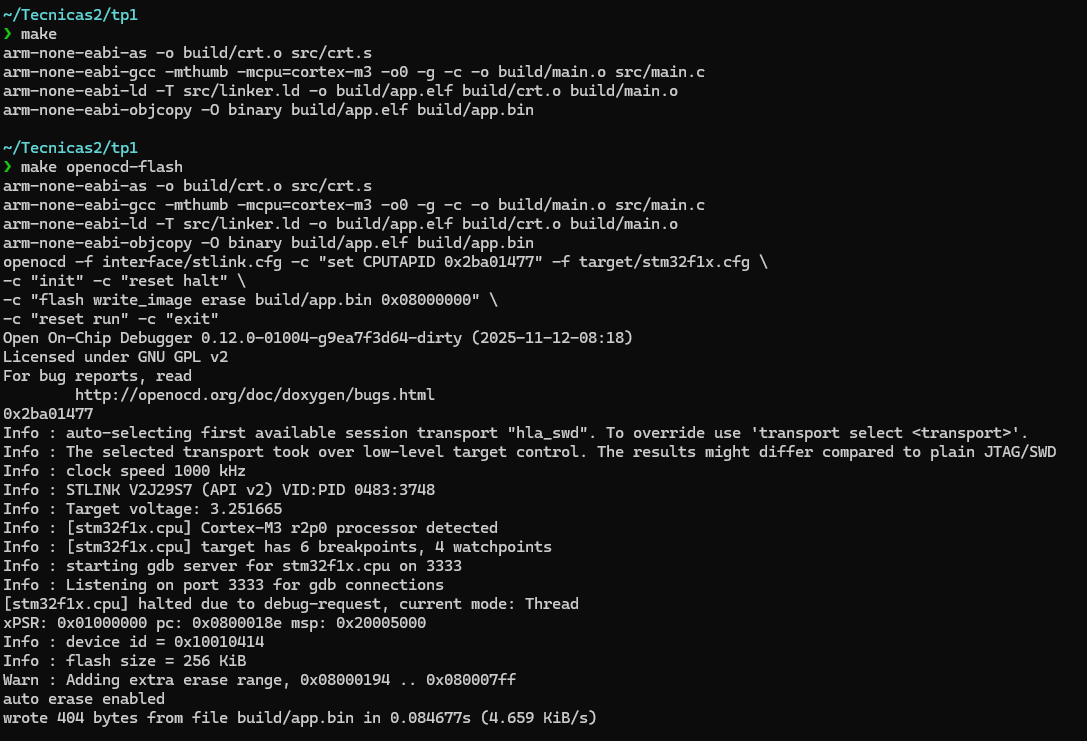
\includegraphics[width=0.5\textwidth]{images/compilacion.png}
    \caption*{Compilación del proyecto utilizando make}
    \label{fig:compilacion}
\end{figure}
Para el funcionamiento de la placa clon, se tuvieron que cambiar los comandos de programación y depuración, además de modificar el Makefile para añadir dichos comandos y así que funcione de manera correcta.

\raggedbottom

\section{Desarrollo Experimental 1}






\section{Desarrollo Experimental 1}

\section{Conclusión}
Se logró poner en funcionamiento la BluePill, y se logró hacer andar un led usando sus direcciones GPIO. Para esto se tuvo que usar los comandos para la placa clon, ademas de modificar el Makefile para añadir dicho comando y así que funcione de manera correcta. Lo más difícil de este trabajo fue comenzar a pensar el codigo en base a los registros, ya que es un nivel de abstracción al que no estabamos acostumbrados, pero una vez que logramos comprender el funcionamiento del código logramos comprender mejor como funciona un microcontrolador a nivel de hardware, nos resultó particularmente interesante como un programa de alto nivel pasa a ser encender o apagar determinados bits de ciertos registros. 
% Referencias bibliográficas
\section{CODIGOS}

\subsection{main.c}
\begin{lstlisting}[caption={Configuración inicial en main.c}, label={cod:main}]
#include <stdint.h>
// register address
#define RCC_BASE 0x40021000
#define GPIOC_BASE 0x40011000
#define GPIOA_BASE 0x40010800
#define RCC_APB2ENR *(volatile uint32_t *)(RCC_BASE + 0x18)
#define GPIOC_CRH *(volatile uint32_t *)(GPIOC_BASE + 0x04)
#define GPIOA_CRL *(volatile uint32_t *)(GPIOA_BASE + 0x00)
#define GPIOC_ODR *(volatile uint32_t *)(GPIOC_BASE + 0x0C)
#define GPIOA_ODR *(volatile uint32_t *)(GPIOA_BASE + 0x0C)
// bit fields
#define RCC_IOPCEN (1 << 4)
#define RCC_IOPAEN (1 << 2)
#define GPIOC13 (1UL << 13)
#define GPIOA7 (1UL << 7)
// --- Registros del SysTick (Cortex-M Core) ---
#define SysTick_BASE 0xE000E010
#define SysTick_CTRL *(volatile uint32_t *)(SysTick_BASE + 0x00)
#define SysTick_LOAD *(volatile uint32_t *)(SysTick_BASE + 0x04)
#define SysTick_VAL  *(volatile uint32_t *)(SysTick_BASE + 0x08)
// Bits de control de SysTick
#define SysTick_CTRL_ENABLE    (1 << 0) // Habilita el contador
#define SysTick_CTRL_TICKINT   (1 << 1) // Habilita la interrupción de SysTick
#define SysTick_CTRL_CLKSOURCE (1 << 2) // Fuente de reloj
#define SysTick_CTRL_COUNTFLAG (1 << 16) // Bandera de desborde
volatile uint32_t tick;
// función que atiende la interrupción
void SysTick_Handler(void)
{
    tick++;
}
// inicialización del systick
void systick_init_ms(void)
{
    tick = 0;
    SysTick_CTRL &= ~SysTick_CTRL_CLKSOURCE; // Reloj de SysTick a HCLK/8 (8MHz / 8 = 1MHz -> 1 tick = 1us)
    SysTick_LOAD = 999; // Poner valor de RECARGA para 1000 ticks (1ms) (1000 - 1) = 999
    SysTick_VAL = 0; // reset del contador
    SysTick_CTRL |= SysTick_CTRL_TICKINT | SysTick_CTRL_ENABLE; // Habilitar la interrupción de SysTick (TICKINT) Y el contador (ENABLE)
}
// función delay 
void delay_ms_bloqueante(uint32_t ms)
{
    uint32_t tiempo_inicio = tick + ms;
    // Espera activa hasta que el contador global haya avanzado 'ms' milisegundos
    while (tick != tiempo_inicio) ;
}
void main(void)
{
    RCC_APB2ENR |= RCC_IOPCEN;
    RCC_APB2ENR |= RCC_IOPAEN;
    GPIOC_CRH &= 0xFF0FFFFF;
    GPIOC_CRH |= 0x00200000;
    GPIOA_CRL &= 0x0FFFFFFF;
    GPIOA_CRL |= 0x20000000;
    systick_init_ms();
    while (1)
    {
        
        GPIOC_ODR &= ~GPIOC13;
        delay_ms_bloqueante(500); 
        GPIOC_ODR |= GPIOC13;
        delay_ms_bloqueante(500); 

        GPIOA_ODR |= GPIOA7;                  
        delay_ms_bloqueante(500);              
        GPIOA_ODR &= ~GPIOA7;                 
        delay_ms_bloqueante(500);              

    }
}
\end{lstlisting}
\subsection{crt.s}
\begin{lstlisting}[language=ARMasm]
.syntax unified 
.cpu cortex-m3
.thumb
.extern _esstack

.section .text.manejadores // definimos la seccion text.manejadores 

// función básica para manejar los punteros 
.thumb_func 
.weak Default_Handler
Default_Handler:
    b .             /* Bucle infinito */

// definir los vectores ejemplo
.weak NMI_Handler
.thumb_set NMI_Handler, Default_Handler
.weak SysTick_Handler
.thumb_set SysTick_Handler, Default_Handler
.weak HardFault_Handler
.thumb_set HardFault_Handler, Default_Handler

// vectores 
.section .isr_vector,"a",%progbits
.word _esstack
.word _reset
.word NMI_Handler         /* 2:  NMI (Non-Maskable Interrupt) */
.word HardFault_Handler   /* 3:  HardFault (falla grave) */
.word 0                   /* 4:  MemManage (falla de memoria) */
.word 0                   /* 5:  BusFault (falla de bus) */
.word 0                   /* 6:  UsageFault (falla de uso) */
.word 0                   /* 7:  Reservado */
.word 0                   /* 8:  Reservado */
.word 0                   /* 9:  Reservado */
.word 0                   /* 10: Reservado */
.word 0                   /* 11: SVCall (Llamada al Supervisor) */
.word 0                   /* 12: Debug Monitor */
.word 0                   /* 13: Reservado */
.word 0                   /* 14: PendSV (Interrupción pendiente del sistema) */
.word SysTick_Handler     /* 15: El handler del SysTick */

// declaramos la función _reset dentro de la seccion text.reset
.section .text.reset
.thumb_func
.global _reset
_reset:
    bl main
    b .
\end{lstlisting}
\subsection{linker.ld}

\begin{lstlisting}[language=Linker]
MEMORY
MEMORY
{
  FLASH (rx) : ORIGIN = 0x08000000, LENGTH = 64K
  RAM (xrw)  : ORIGIN = 0x20000000, LENGTH = 20K
}

/* 2. Definición de Símbolos Globales */
ENTRY(_reset) /* El punto de entrada, definido en tu crt.s */

/* Símbolo para el final de la pila, usado en tu .isr_vector */
_esstack = ORIGIN(RAM) + LENGTH(RAM); /* 0x20005000 (el final de los 20K de RAM) */

/* 3. Definición de las Secciones de Salida */
SECTIONS
{
  /* SECCIONES EN FLASH */
  /* La tabla de vectores debe ir primero en la Flash */
  .isr_vector :
  {
    KEEP(*(.isr_vector))  /* Mantiene la sección .isr_vector de tu crt.s */
  } > FLASH

  /* Código del programa y datos de solo lectura */
  .text :
  {
    *(.text)             /* Todo el código C y ensamblador */
    *(.text*)            /* Variantes de .text */
    *(.rodata)           /* Datos de solo lectura (constantes) */
    *(.rodata*)
  } > FLASH
  /* SECCIONES EN RAM */
  /* .data: Variables inicializadas con un valor distinto de cero (ej: int x = 10;) */
  /* El linker necesita símbolos para que el startup mueva los datos */
  _sidata = LOADADDR(.data); /* Dirección de los valores en FLASH */

  .data :
  {
    _sdata = .;           /* Inicio de .data en RAM */
    *(.data)
    *(.data*)
    _edata = .;           /* Fin de .data en RAM */
  } > RAM AT> FLASH     /* Ubicada en RAM, pero cargada desde FLASH */
  /* .bss: Variables inicializadas a cero o sin inicializar */
  /* (ej: static int y; o int z = 0;) */
  .bss :
  {
    _sbss = .;            /* Símbolo de inicio de .bss */
    *(.bss)
    *(.bss*)
    *(COMMON)
    _ebss = .;            /* Símbolo de fin de .bss */
  } > RAM               /* Solo ocupa espacio en RAM */
}

\end{lstlisting}

\subsection{makefile}
\begin{lstlisting}[language=MyMake]
SRC_DIR = src
BUILD_DIR = build
CC = arm-none-eabi-gcc
AS = arm-none-eabi-as
LD = arm-none-eabi-ld
BIN = arm-none-eabi-objcopy
CFLAGS = -mthumb -mcpu=cortex-m3 -o0 -g

all: app.bin

$(BUILD_DIR):
	mkdir $(BUILD_DIR)

crt.o: $(BUILD_DIR) $(SRC_DIR)/crt.s
	$(AS) -o $(BUILD_DIR)/crt.o $(SRC_DIR)/crt.s

main.o: $(BUILD_DIR) $(SRC_DIR)/main.c
	$(CC) $(CFLAGS) -c -o $(BUILD_DIR)/main.o $(SRC_DIR)/main.c

app.elf: $(BUILD_DIR) $(SRC_DIR)/linker.ld crt.o main.o
	$(LD) -T $(SRC_DIR)/linker.ld -o $(BUILD_DIR)/app.elf $(BUILD_DIR)/crt.o $(BUILD_DIR)/main.o 

app.bin: app.elf
	$(BIN) -O binary $(BUILD_DIR)/app.elf $(BUILD_DIR)/app.bin

clean:
	rm -rf $(BUILD_DIR)

openocd-flash: app.bin
	openocd -f interface/stlink.cfg -c "set CPUTAPID 0x2ba01477" -f target/stm32f1x.cfg \
	-c "init" -c "reset halt" \
	-c "flash write_image erase $(BUILD_DIR)/app.bin 0x08000000" \
	-c "reset run" -c "exit"

openocd-erase:
	openocd -f interface/stlink.cfg -c "set CPUTAPID 0x2ba01477" -f target/stm32f1x.cfg \
	-c "init" -c "reset halt" \
	-c "flash erase_sector 0 0 last" -c "reset run" -c "exit"

\end{lstlisting}


\end{document}